% Dados: dados/validacoes_2026-10-19.csv (execução de 19/10/2026, 29 planos)
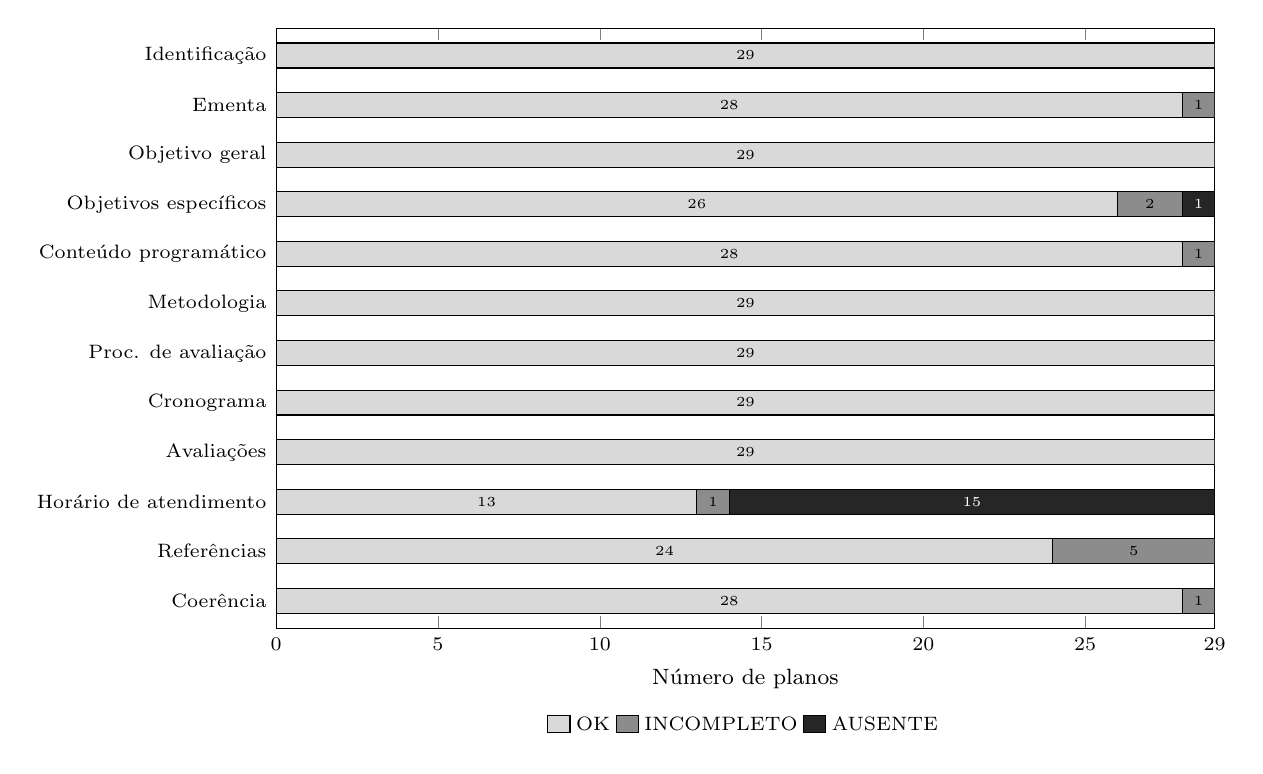
\begin{tikzpicture}
\begin{axis}[
  xbar stacked,
  width=13.5cm, height=9.2cm,
  bar width=9pt,
  xmin=0, xmax=29,
  xtick={0,5,10,15,20,25,29},
  xlabel={Número de planos},
  ytick=data,
  yticklabels={Identificação,Ementa,Objetivo geral,Objetivos específicos,Conteúdo programático,Metodologia,Proc. de avaliação,Cronograma,Avaliações,Horário de atendimento,Referências,Coerência},
  y dir=reverse,
  ticklabel style={font=\scriptsize},
  label style={font=\footnotesize},
  legend style={at={(0.5,-0.13)}, anchor=north, legend columns=3, font=\scriptsize, draw=none},
  nodes near coords={\pgfmathprintnumber{\pgfplotspointmeta}},
  nodes near coords style={font=\tiny},
  point meta=explicit symbolic,
  enlarge y limits=0.05,
]
\addplot[fill=black!15, draw=black] coordinates {
  (29,1) [29] (28,2) [28] (29,3) [29] (26,4) [26] (28,5) [28] (29,6) [29]
  (29,7) [29] (29,8) [29] (29,9) [29] (13,10) [13] (24,11) [24] (28,12) [28]};
\addplot[fill=black!45, draw=black] coordinates {
  (0,1) [] (1,2) [1] (0,3) [] (2,4) [2] (1,5) [1] (0,6) []
  (0,7) [] (0,8) [] (0,9) [] (1,10) [1] (5,11) [5] (1,12) [1]};
\addplot[fill=black!85, draw=black, nodes near coords style={font=\tiny, text=white}] coordinates {
  (0,1) [] (0,2) [] (0,3) [] (1,4) [1] (0,5) [] (0,6) []
  (0,7) [] (0,8) [] (0,9) [] (15,10) [15] (0,11) [] (0,12) []};
\legend{OK, INCOMPLETO, AUSENTE}
\end{axis}
\end{tikzpicture}
